\chapter{Methodology}
\label{ch:methodology}

\newpage
\section{Synthetic Techniques}\label{s:synthetic}

In the context of porous carbon materials, activation is the process of porosity development in carbonaceous material.\citep{Sevilla2014Energy} In this work, activation is principally conducted \textit{via} chemical oxidation,\citep{Sevilla2014Energy} that is by the oxidative action of a caustic agent - either \ce{KOH} (chapter \ref{ch:cbs} and \ref{ch:impregnation}) or the self-activation of a polymer containing \ce{Na+} ions (chapter \ref{ch:impregnation}) - on the carbon framework of the precursor. The oxidation of \ce{C} to \ce{CO2} and/or \ce{CO3^2-} results in voids forming in the semi-graphitic structure.\citep{Wang2009High, Wang2012, Otowa1993Production} Further pore-forming processes may include intercalation of free \gls{porogen} ions between graphitic layers,\citep{LozanoCastello2007Carbon} as well as the formation of cross-links between polymeric chains prior to carbonisation.\citep{lin2015preparation, yu2017koh, yu2017one}

\Gls{htc} is often used in the synthesis of \glspl{turbostratic carbon} to make the precursor easier to activate. The process consists of simply placing a mixture of the precursor (typically biomass) and water into a sealed vessel and heating to temperatures between 180 and \qty{300}{\degreeCelsius}. The ease of activation is attributed to the solid product, known as \gls{hydrochar}, having a high \ce{O} content and low aromaticity.\citep{Sevilla2011Hydrothermal, Sevilla2009Chemical, Sevilla2009a} Indeed, the interaction with water molecules results in the formation of microspheres with a hydrophobic core and hydrophilic shell; this means that any \gls{porogen} used in a subsequent activation step has much greater contact with these \ce{O}-rich moieties.

\begin{table}[ht!]
    \caption{Synthetic details of samples derived from cigarette butts.}
    \label{tb:cb_synthesis}
    \begin{tabularx}{\textwidth}{lXl}
        \toprule
            \textbf{Prefix} & \textbf{Preparation}  & \textbf{\# Samples} \\ 
        \midrule
            \textbf{hC}     & From public ash tray; Ash, excess tobacco removed before grinding. \Gls{hydrochar} washed with \qty{500}{\cm\cubed} water.  & 9              \\
            \textbf{hD}     &  From public ash tray; Ash, excess tobacco removed before grinding. & 9             \\
            \textbf{hE}     & Single brand from single smoker. Paper, ash, excess tobacco removed before grinding.  & 3              \\
        \bottomrule
    \end{tabularx}%
\end{table}

In chapter \ref{ch:cbs} activated carbons were produced from \glspl{ucb} collected from two different sources. Sets C and D came from a public ash tray and were used without removing the wrapping paper. Sets E came from a single brand from a single smoker and the wrapping paper was removed before further treatment. Full details of the sample sets can be found in table \ref{tb:cb_synthesis}. In all cases, \qty{2.5}{\gram} \acrshortpl{ucb} were ground in a spice grinder before being hydrothermally carbonised with \qty{25}{\cm\cubed} water in a teflon-lined stainless steel autoclave by heating at \qty{5}{\degreeCelsius\per\minute} to \qty{250}{\degreeCelsius}. Temperature was held for \qty{2}{\hour} before the reaction mixture was allowed to cool to ambient temperature. Samples in set C were washed with \qty{500}{\cm\cubed} water under suction to attempt remove any contaminants, while others (sets D and E) were derived without this treatment. In either case, the resultant \glspl{hydrochar} was dried for at \qty{100}{\degreeCelsius} for \qty{24}{\hour}. \Gls{hydrochar} was then activated, either with \ce{KOH} or alone in a tube furnace under \ce{N2} at a flow rate of \qty{60}{\cm\cubed\per\minute} by heating at a rate of \qty{3}{\degreeCelsius\per\minute} to the target temperature (\qtylist[list-units=single, list-final-separator={ or }]{600;700;800}{\degreeCelsius} and holding for \qty{1}{\hour}. After being allowed to cool, all samples activated with \ce{KOH} were washed in \qty{600}{\cm\cubed} of \qty{10}{\volpercent} \ce{HCl} solution for at least \qty{24}{\hour}, then filtered and washed with water to give neutral washings. A portion of the samples activated without \ce{KOH} were not washed in order to examine the effect of the washing step on the composition, morphology and porosity of the resultant samples. Sample designation is h\textit{A-xTTT}, where h indicates the \gls{htc} step, \textit{A} is the sample prefix (see table \ref{tb:cb_synthesis}), \textit{x} is KOH:\acrshort{ucb} ratio (wt./wt.), and \textit{TTT} is activation temperature in \unit{\degreeCelsius}. For the self activated samples i.e. those that did not use \ce{KOH} in the activation step, $'$ is appended to the end to indicate those which were not washed. For example hC-0800$'$ indicates a sample activated at \qty{800}{\degreeCelsius} in the absence of \gls{activating agent}, and that was not washed. To refer to the \gls{hydrochar} itself, the designation is h\textit{A}-hydrochar, e.g. \gls{hydrochar} derived from \acrshort{ucb}-\gls{hydrochar} set hD (see table \ref{tb:cb_synthesis}) is hD-hydrochar.


Sawdust-derived carbons were made in chapter \ref{ch:impregnation} by incorporating \ce{KOH} at the \gls{htc} step. An aqueous solution of \ce{KOH} was made where the mass of the \ce{KOH} was defined as a ratio (between \numrange{0.00}{2.00}) of the mass of the sawdust used. The solution was then mixed with the sawdust and placed in an autoclave. The autoclave and contents were heated at a ramp rate of \qty{5}{\degreeCelsius} to the target temperature (\qtylist[list-units=single, list-final-separator={ or }]{200;250;300}{\degreeCelsius}), held for \qty{2}{\hour} and then allowed to cool. The procedure was completed by drying the resultant slurry overnight at \qty{100}{\degreeCelsius} and then activating in a tube furnace under \ce{N2} (\qty{60}{\cm\cubed\per\minute}) at \qty{800}{\degreeCelsius} for \qty{1}{\hour} following a ramp rate of \qty{3}{\degreeCelsius\per\minute}. These sawdust-derived carbons are designated SA\textit{x.xx-HHH} where the prefix SA indicates activated sawdust, \textit{x.xx} is the KOH:sawdust ratio and \textit{HHH} is the \gls{htc} temperature. All samples were washed with\qty{600}{\cm\cubed} of \qty{10}{\volpercent} \ce{HCl} solution for a minimum of \qty{24}{\hour} before being filtered under suction and washed with water until the pH of the washings was neutral. Finally the samples were dried at \qty{100}{\degreeCelsius} overnight. The hydrothermally carbonised intermediates were also isolated and washed with water (\qty{500}{\cm\cubed}) under suction before drying overnight at \qty{100}{\degreeCelsius}. The hydrochars are designated  SH\textit{x.xx-HHH} to differentiate them from the activated samples.

\begin{figure}[ht!]
    \centering
    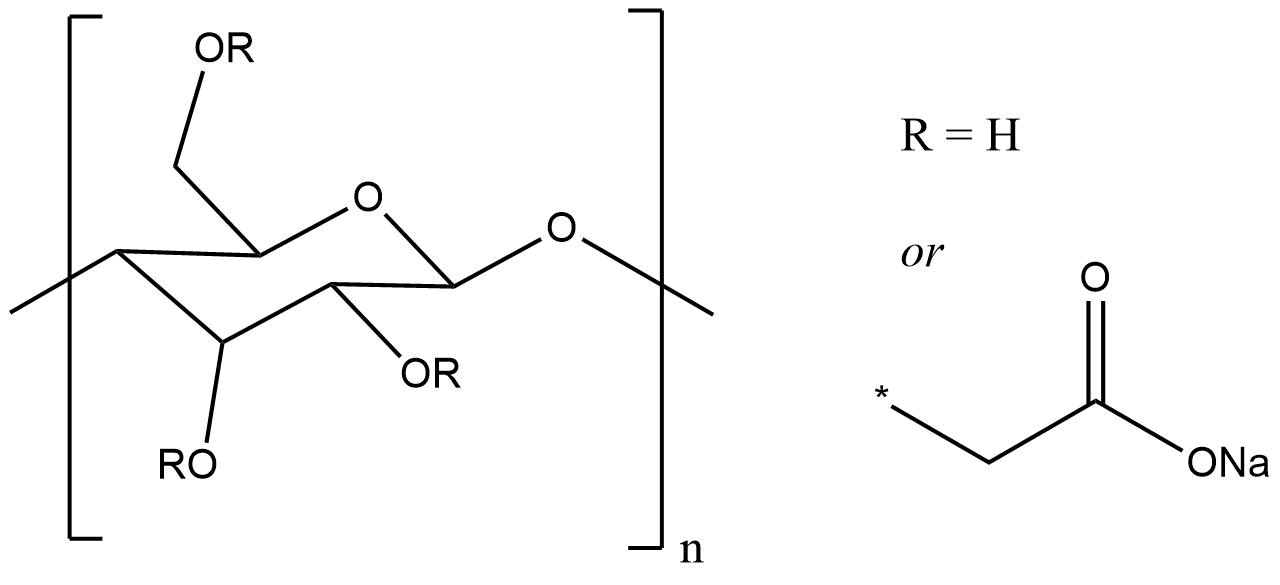
\includegraphics[width=0.8\columnwidth]{4-impregnation/figs/nc_structure.png}
    \caption{Structure of sodium carboxymethyl cellulose. \Acrfull{ds} is taken as the average number of sodium carboxymethyl groups (\ce{-CH2COONa}) per monomer.}
    \label{fig:nc_structure}
\end{figure}

Additionally, in chapter \ref{ch:impregnation} \acrfull{nc} was used as a precursor for direct (without \gls{htc}) activation. The structure of \acrshort{nc} is shown in figure \ref{fig:nc_structure}. Carbons were obtained from \acrshort{nc} with different \acrfullpl{ds} (\qtylist[list-final-separator={ or }, list-units=single]{0.0;0.7;0.9;1.2}), obtained from Sigma-Aldrich. For all samples, NC was heated under a flow of \ce{N2} (\qty{60}{\cm\cubed\per\minute}) at a rate of \qty{3}{\degreeCelsius\per\minute} and held for \qty{1}{\hour} at the target temperature of \qtylist[list-final-separator={ or }, list-units=single]{600;700;800}{\degreeCelsius}. Samples were washed in \qty{600}{\cm\cubed} of \qty{10}{\volpercent} \ce{HCl} solution, before being filtered and washed with deionised water to give neutral washings, and finally dried at \qty{100}{\degreeCelsius} for \qty{24}{\hour}. Samples are designated as NC\textit{x.x-TTT} where \acrshort{nc} indicates sodium carboxymethyl cellulose, \textit{x.x} is the \acrshort{ds}, and \textit{TTT} is the activation temperature. 

\section{Composition and morphology}\label{s:composition_morphology}
Techniques in this section were employed to understand the composition, structure, and porosity of samples synthesised in this work, and their results are presented in chapters \ref{ch:cbs} and \ref{ch:impregnation}. The more precise compositional analysis techniques - \acrfull{xps} and \acrfull{icp-oes} - as well as electron microscopy were only used for samples produced from \acrfullpl{ucb} in chapter \ref{ch:cbs}.

\acrfull{tga} measures the mass of a sample undergoing heating as a function of temperature or time.\citep{coats1963thermogravimetric} \acrshort{tga} was used in this study primarily to determine the \gls{ash content} of samples, thus giving a measure of sample purity,\citep{mcnaught1997compendium} i.e. whether the material contains any non-combustible matter, typically residual metals. For this work, \acrshort{tga} was performed using a TA Q500 Thermogravimetric Analyser. All samples were analysed using a platinum pan under a flow of air at \qty{100}{\cm\cubed\per\min}. All experiments took place as follows; temperature was increased at \qty{10}{\degreeCelsius\per\minute} from ambient to \qty{1000}{\degreeCelsius} before dwelling for \qty{10}{\minute}.

CHN elemental microanalysis precisely determines the concentration (by weight) of carbon, nitrogen and hydrogen that make up a sample. This is achieved by total combustion of the sample at \qty{975}{\degreeCelsius} under pure oxygen. At this stage impurities such as sulfur, phosphorous, and halogen compounds are also removed \textit{via} various reactions. This results in a pure mixture of \ce{H2O}, \ce{CO2} and oxides of nitrogen, which is transferred by means of a flow of He to a reduction chamber where the nitrogen oxides are reduced to \ce{N2}. This mixture of three sample gases plus the He carrier gas is then equilibrated to precise and constant temperature, volume and pressure. \ce{H2O} and \ce{CO2} are then sequentially separated according to their thermal conductivity, leaving a flow of \ce{N2} and \ce{He}. The volumes of \ce{H2O} and \ce{CO2} can then directly be used to calculate the sample \ce{H} and \ce{C} concentrations. The mixture of \ce{N2} and \ce{He} is compared with a reference flow of pure \ce{He} to determine \ce{N} content. For this study, CHN analysis was performed using an Exeter Analytical CE-440 Elemental Analyzer.
% find citation
% particular details of machine.

In general \acrfull{p-xrd} is principally used to identify elements and determine inter-layer spacing within crystalline powder samples. In the case of the partially-ordered \glspl{turbostratic carbon} and \glspl{hydrochar} reported in this thesis \acrshort{p-xrd} was used to determine the extent of graphiticity (i.e. how ordered the turbostratic domains are). In addition sharp peaks indicate the presence of crystalline material, which can be attributed to contaminants - typically residual \gls{porogen}. In this study, \acrshort{p-xrd} measurements were made using a PANalytical X’Pet Pro diffractometer, with \ce{Cu}K\textgreek{α} X-rays of wavelength \qty{1.54}{\angstrom}. Data collection occurred at 2\textgreek{θ} from \qtyrange[range-units=single]{2}{80}{\degree}.

X-ray photoelectron spectra are produced \textit{via} the irradiation of a sample with an X-ray beam, resulting in the ejection of electrons from low energy atomic orbitals according to the photoelectric effect\citep{richardson1912liii}. The electrons are collected and detected by the apparatus, facilitating the elucidation of the identity and quantity of elements present on the surface of the material from the kinetic energy of ejected electrons and the number of electrons ejected at each binding energy, respectively. The binding energy, $E_B$ is calculated according to the below equation;

\begin{equation}\label{eq:xps}
    E_B = h\nu - \Phi - E_K
\end{equation}

where $h\nu$ is the photon energy, $\Phi$ is the sample’s work function, and $E_K$ is the kinetic energy of the photoelectron. So-called `shifting' of elemental characteristic $E_B$ from those expected according equation \ref{eq:xps} can be used to determine chemical and electronic states of detected species.\citep{moulder1995handbook} For the purpose of \acrshort{xps} analysis in this work, samples were prepared from selected \glspl{hydrochar} and \glspl{turbostratic carbon} by performing a \acrshort{tga} in air to burn off all carbonaceous material. The remaining inorganic matter was then analysed using the Kratos AXIS ULTRA with a mono-chromated \ce{Al}k\textgreek{α} X-ray source (\qty{1486.6}{\electronvolt}) operated at \qty{10}{\mA} emission current and \qty{12}{\kilo\volt} anode potential (\qty{120}{\watt}). Spectra were acquired with the Kratos VISION II software. A charge neutralizer filament was used to prevent surface charging. Hybrid–slot mode was used measuring a sample area of approximately \qtyproduct{300 x 700}{\micro\metre}. The analysis chamber pressure was better than \qty{5e-9}{\milli\bar}. Three areas per sample were analysed. A wide scan at low resolution (Binding energy range \qtyrange{1400}{-5}{\electronvolt}, with pass energy \qty{80}{\electronvolt}, step \qty{0.5}{\electronvolt}, sweep time \qty{20}{\minute}) was used to estimate the total atomic \% of the detected elements. High resolution spectra at pass energy \qty{20}{\electronvolt}, step of \qty{0.1}{\electronvolt}, and sweep times of \qty{10}{\minute} each were also acquired for photoelectron peaks from the detected elements and these were used to model the chemical composition. The spectra were charge corrected to the C 1s peak set to \qty{285}{\electronvolt}. Casaxps (version 2.3.19 PR1.0) software\citep{fairley2021systematic} was used for quantification and spectral modelling.

Optical Emission Spectrometry (OES), also known as Atomic Emission Spectrometry (AES) is a technique used to quantify concentration of elements in solution by exciting them and measuring intensity of emissions at some characteristic wavelength associated with the return of the species to the ground state. These intensities are then converted to concentrations using a calibration curve. While there are multiple methods to excite the atoms, a common method is using Inductively Coupled Plasma (ICP) which also acts to separate elements in the solution. This technique is thus abbreviated to \acrshort{icp-oes} or ICP-AES.\citep{Hinners1988interlaboratory} In this work, samples were prepared for \acrshort{icp-oes} by dry-ashing in an alumina crucible at \qty{600}{\degreeCelsius} for at least \qty{16}{\hour}, the ash was then digested in an aqueous solution of \qty{10}{\volpercent} each of high purity \ce{HNO3} and \ce{HCl} (Aristar grade). The mixture was then sonicated for several hours, and digestion was completed via microwave, before being centrifuged at \qty{4000}{rpm} for \qty{99}{\minute}. Finally the digestate was filtered through syringe filters to remove any remaining sediment. References and blanks were prepared from the same stock digestion solution to ensure consistency. Standards were made from a 28-element standard (\qty{100}{\mg\per\dm\cubed}, \qty{2}{\volpercent} \ce{HNO3} matrix from Fisher) at concentrations of \qtylist[list-units = single]{0.1;1;10;50;100}{\mg\per\dm\cubed}. Measurements were made using a Perkin-Elmer Optima 2000 Spectrometer, using argon plasma.

\subsection{Electron microscopy}

Various forms of electron microscopy were used on the samples in chapter \ref{ch:cbs} in order to determine sample morphology as well as composition and dispersion of inorganic heteroatoms. The principal types are detailed here.

\paragraph{\acrfull{sem}} uses a beam of focused electrons in order to image solid materials. As the electrons interact with the material, electrons and electromagnetic radiation are emitted via various mechanisms. \Acrfull{se} are a result of the ejection of electrons from atoms near the sample surface, and \acrfull{sei} provide high resolution images of surface morphology and texture.\citep{Goldstein2017Scanning} 

\paragraph{\acrfull{bse}} are electrons deflected by nuclear electrostatic charge – degree of deflection increases with nuclear charge. Though this results in much lower resolution images, \acrfull{bed} images the material according to atomic weight, with heavier elements showing up as bright spots. This technique does not identify elements, but can be used to map heavier elements interspersed within a low atomic mass material.\citep{Goldstein2017Scanning}

\paragraph{\acrfull{tem}} differs from \acrshort{sem} in that the electrons are transmitted through the sample as opposed to reflecting off of it. Imaging with \acrshort{tem} allows for much more detailed imaging, down to the atomic scale.\citep{knoll1932elektronenmikroskop}

\paragraph{\acrfull{edx}} relies on the excitation by X-rays of electrons within a sample to identify and quantify its elemental components. It can be coupled with \acrshort{tem} in order to image the dispersion of elements within a sample, this technique is known as \acrshort{edx}-\acrshort{tem}.\citep{Goldstein2017Scanning}

In this work, \acrshort{sem} images were taken on a JEOL 7100F FEG-SEM with detector set at a working distance of 10.00 mm. SE images were captured with an electron accelerating voltage of 1.00 or 2.00 kV, but this was increased to 15.00 kV for \acrshort{bse}. \acrshort{tem} images were taken on a JEOL 2100F FEG-TEM, with elemental dispersion determined using the \acrshort{edx} attachment.

\section{Isotherms}\label{s:porosimetry}

In this work isotherms were measured in order to determine the porosity of the carbon samples as well as to find ambient temperature gravimetric \ce{CO2} uptake capacity as a function of pressure. The techniques used for these measurements are discussed below.

All \ce{N2} isotherms used for porosimetry were measured at \qty{-196}{\degreeCelsius} on a 3flex analyser from Micromeritics. Prior to isotherm measurement, all samples were degassed at \qty{300}{\degreeCelsius} for \qty{16}{\hour} under high vacuum. Adsorption were then measured in the relative pressure range \numrange{\sim e-8}{\sim1}, after which the desorption isotherm was measured down to \num{\sim0.1}. Thereafter free space was measured using \ce{He} at both ambient and analysis temperature and used to adjust the previously measured isotherm. From the isotherms, $A_{BET}$ values were determined using the Rouquerol method in the case of type-I isotherms,\citep{Rouquerol2007Is} otherwise this value was calculated using the linear portion of the BET transform within relative pressures between 0.05 and 0.30. Total pore volume ($V_t$) was determined from the volume adsorbed by the sample at a single point at relative pressure \num{\sim0.9} on the plateau of the isotherm. Classical determination of \gls{micropore} volume and surface area were determined using t-plot, with a carbon black STSA thickness curve. All \acrshortpl{psd} are derived using the 2D-NLDFT heterogeneous surface kernel in the SAIEUS software,\citep{Jagiello20132D} with the regularization parameter, $\lambda$\citep{Hansen1992Analysis, Hansen2001L} kept constant for samples derived from the same precursor and chosen to optimise fit across all isotherms. 

While the porosimetric analyses in chapters \ref{ch:cbs} and \ref{ch:impregnation} use only \ce{N2} isotherms, in chapters \ref{ch:dual_isotherm} and \ref{ch:pyPUC}  \ce{O2} and \ce{H2} isotherms measured at \qty{-196}{\degreeCelsius} were used to improve porosimetric analysis. \ce{O2} isotherms were measured in the same manner as for \ce{N2}, however \ce{H2} isotherms were measured up to  the arbitrary pressure of \qty{1013}{\milli\bar} as \ce{H2} is supercritical at \qty{-196}{\degreeCelsius} and thus relative pressure is not physically meaningful. In chapter \ref{ch:dual_isotherm}, the same classical measures of porosity were calculated from \ce{O2} isotherms as previously performed using \ce{N2} isotherms. Comparisons were made of the \acrshortpl{psd} derived from fitting 2D-NLDFT heterogeneous surface kernels to \ce{O2}, \ce{N2}, and \ce{H2} isotherms. In addition, Jagiello's multiple isotherm fitting procedure\citep{Jagiello2015Dual} was employed with combinations of \ce{N2}, \ce{O2} and \ce{H2} isotherms to yield a single \acrshort{psd} for a single sample. These porosities derived from these alternative techniques were compared in \ref{ch:dual_isotherm}, and further used to assess the relationship between porosity and low-pressure \ce{CO2} uptake in chapter \ref{ch:pyPUC}.

Excess \ce{CO2} uptake isotherms of \gls{turbostratic carbon} samples reported in chapters \ref{ch:cbs} and \ref{ch:pyPUC} was determined \textit{via} gravimetric analysis. This begins with the degassing of the samples under vacuum followed by precise measurement of the weight of the sample with increasing \ce{CO2} pressure. The procedure results in an excess \ce{CO2} uptake isotherm, from which molar gravimetric uptake can be read as a function of pressure. Measurements were taken at either \qtylist[list-pair-separator={ or }, list-units=single]{25;18}{\degreeCelsius} and up to \qtylist[list-pair-separator={ or }, list-units=single]{40;20}{\bar}, on XEMIS or IGA analysers respectively from Hiden Isochema. 

\section{Software development}
Chapter \ref{ch:pyPUC} describes the use of several python libraries in order to calculate linear regressions between porosity within some range of pore sizes to uptake of \ce{CO2} at some pressure. The main libraries used in this project, known as the python Porosity Uptake Correlator (pyPUC) are \verb|scipy|,\citep{SciPy2020} \verb|numpy|,\citep{numpy2022} \verb|pandas|,\citep{pandas2010} and \verb|pygaps|.\citep{Iacomi2019pyGAPS}

pyPUC is a fairly simple package whose structure is shown in figure \ref{fig:pyPUC_structure}. It is written almost exclusively in python,\citep{python1995} apart from one small bash script.\citep{bash2007} The main functions of pyPUC can be found in \verb|pyPUC/pyPUC/core|, while outside of this is the module \verb|pyPUC/interface.py| which constructs a simple command line interface to run the program, and the bash script \verb|pyPUC-cli| which executes \verb|pyPUC/interface.py|. Finally there is a directory for the \verb|source_data| which should be populated by the user with \acrshortpl{psd} and experimental uptake isotherms for the project in question.

\begin{figure}[ht!]
    \centering
    \begin{forest}
          for tree={
            font=\ttfamily,
            grow'=0,
            child anchor=west,
            parent anchor=south,
            anchor=west,
            calign=first,
            inner xsep=7pt,
            edge path={
              \noexpand\path [draw, \forestoption{edge}]
              (!u.south west) +(7.5pt,0) |- (.child anchor) pic {folder} \forestoption{edge label};
            },
            % style for your file node 
            file/.style={edge path={\noexpand\path [draw, \forestoption{edge}]
              (!u.south west) +(7.5pt,0) |- (.child anchor) \forestoption{edge label};},
              inner xsep=2pt,font=\small\ttfamily
                         },
            before typesetting nodes={
              if n=1
                {insert before={[,phantom]}}
                {}
            },
            fit=band,
            before computing xy={l=15pt},
          }  
        [pyPUC
          [pyPUC
            [core
              [best\_width\_at\_pressure.py,file]
              [psd\_processing.py,file]
              [uptake\_processing.py,file]
              [utils.py,file]
            ]
            [interface.py,file]
          ]
          [source\_data
            [project
              [psd
                [sorptive(s)]
              ]
              [uptake
                [sorptive]
              ]
            ]
          ]
          [pyPUC-cli,file]
        ]
    \end{forest}
    \caption{Structure of key modules and directories in the pyPUC package. There are other components in the github repository but they are not essential to the function of the package.}
    \label{fig:pyPUC_structure}
\end{figure}

The code is well documented, however a brief discussion of the purpose of each of the modules in \verb|pyPUC/pyPUC/core| follows here. Firstly \verb|utils.py| defines utility methods for the other three modules. Most important are the methods \verb|read_data()| and \verb|define_array()|. The former simply reads the data from the \verb|source_data| directory according to input arguments using the \verb|pandas| library,\citep{pandas2010} while the latter is a simple method for defining an array of pressures or pore widths for the modules \verb|uptake_processing| or \verb|psd_processing| using the \verb|numpy| library.\citep{numpy2022} 

The \verb|uptake_processing.py| and \verb|psd_processing.py| modules are fairly self-explanatory, in each case simply processing the uptake or \acrshort{psd} data for all samples in \verb|source_data/project|. The outputs from these modules can be seen in figure \ref{tb:loading_param_outputs}. The former attempts to fit each uptake isotherm in the appropriate project in \verb|source_data| to a range of model isotherms and selects the best fit, by using the \verb|modelling| module from the library \verb|pygaps|.\citep{Iacomi2019pyGAPS} These model isotherms are then converted to point isotherms at pressures defined by the user. The pressures and loadings are then stored in a two-dimensional DataFrame, $D_\upsilon$ (see table \ref{tb:loading_output}). The latter reads in the cumulative \acrshortpl{psd} for each sample, and determines the pore volume or surface area within each user-defined pore size range. A demonstration of how this works is shown in figure \ref{fig:pypuc_porosity}. This is done for each sample and stored in the DataFrame $D_\pi$ (see table \ref{tb:param_output}). In either case, the data produced can be stored in memory or output as a \verb|.csv|, alongside a simple report of the data processing (see appendix figures \ref{fig:loading_report} and \ref{fig:psd_report}).

\begin{table}[t!]
\centering
\captionof{table}{An example output of processed data from the \texttt{uptake\_processing.py} (a) and \texttt{psd\_processing.py} modules (b). \textit{A}, \textit{B}, \textit{C}, and \textit{D} are the four samples used in this analysis. In the case of (a), the numbers are the loadings of \ce{CO2} on the samples at each of the pressures in column \textit{p}, and for (b) they are the surface areas of the samples within the pore size range defined by $w_{min}$ and $w_{max}$.}
    \begin{subtable}{.5\linewidth}
      \centering
        \caption{}
        \begin{tabular}{l|l|l|l|l}
            p & A & B & C & D \\
            \midrule
            1 & 4.27 & 4.01 & 4.27 & 4.35 \\
            2 & 5.93 & 5.25 & 5.93 & 5.95 \\
            3 & 6.94 & 5.96 & 6.94 & 6.91 \\
        \end{tabular}
    \label{tb:loading_output}
    \end{subtable}%
    \begin{subtable}{.5\linewidth}
      \centering
        \caption{}
        \begin{tabular}{l|l|l|l|l|l}
            $\rm w_{min}$ & $\rm w_{max}$ & A & B & C & D \\
            \midrule
            5 & 4 & 59 & 282 & 238 & 260 \\
            6 & 4 & 401 & 514 & 442 & 465 \\
            6 & 5 & 142 & 232 & 204	& 204 \\
        \end{tabular}
    \label{tb:param_output}
    \end{subtable} 
\label{tb:loading_param_outputs}

\vspace{10pt}
\begin{python}
import pandas as pd
import numpy as np

sample_df = pd.read_csv('psd.csv')  # PSD stored in DataFrame 
w_array = [4, 5, 6]  # array of pore widths  
i=0
for wmax in w_array[1:]:  
    for wmin in w_array[w_array<wmax]:  # every possible combination of two w values
        rows_max = np.max(list(np.where(w < wmax)))
        rows_min = np.min(list(np.where(w > wmin)))
        max_value = sample_df.loc[rows_max, 'Vcum']
        min_value = sample_df.loc[rows_min, 'Vcum']
        param = max_value - min_value
        i+=1 # Go through all possible values of wmin for wmax
\end{python}
\captionof{figure}{How the porosity within some pore width range is determined in pyPUC. Note that this is pseudo-code\citep{davis2019pseudocode} as opposed to the actual source code.}
\label{fig:pypuc_porosity}
\end{table}

Finally \verb|best_width_at_pressure.py| takes the two DataFrames generated by \verb|uptake_processing.py| and \verb|psd_processing.py| and uses the \verb|stats.linregress()| method from the \verb|scipy| library\citep{SciPy2020} to perform linear regressions between each row of $D_\upsilon$ and each row of $D_\pi$. That is, if each of $D_\upsilon$ and $D_\pi$ have three rows (1, 2, 3) then a linear regression of row 1 in $D_\upsilon$ will be performed against each row 1, 2 and 3 of $D_\pi$. Then the same is performed for row 2 of $D_\upsilon$, etc.. \verb|scipy.stats.linregress()| then returns the $r^2$ value, slope, and intercept of the regression which is stored in the correlation DataFrame, $D_c$ alongside the values for $w_{min}$, $w_{max}$ and $P$ - an example of this can be seen in table \ref{tb:D_c}. $D_c$ can be reduced in size using the method \verb|correlation_requirements()| which allows rows in the DataFrame to be eliminated according to various arguments. The best pair of $w_{min}$ and $w_{max}$, according to the highest $r^2$ value for each pressure can be selected using the method \verb|make_correlation_df()|, i.e. yielding the optimum pore size region for uptake of the sorptive, $\Omega$.

\begin{table}[t!]
    \centering
    \begin{tabular}{l|l|l|l|l|l|l|l}
        $\rm w_{min}$ & $\rm w_{max}$ & p & $\rm r^2$ & m & c & x & y \\
        \midrule
        \rowcolor{yellow} 4 & 5 & 1 & 0.503 & -0.005 & 5.77 & [259 282 ...] & [4.27 4.01 ...] \\
        \rowcolor{yellow} 4 & 5 & 2 & 0.667 & -0.0157	& 9.85 & [259 282 ...] & [5.93 5.25 ...] \\
        4 & 5 & 3 & 0.691 & -0.0225 & 12.5 & [259 282 ...] & [6.94 5.96 ...] \\
        4 & 6 & 1 & 0.457 & -0.00213 & 5.20 & [401 514 ...] & [4.27 4.01 ...] \\
        4 &	6 & 2 & 0.662 & -0.00591 & 8.46	& [401 514 ...] & [5.93 5.25 ...] \\
        \rowcolor{yellow} 4 & 6 & 3 & 0.696 & -0.00854 & 10.5 & [401 514 ...] & [6.94 5.96 ...] \\
        5 & 6 & 1 & 0.254 & -0.00196 & 4.61 & [142 232 ...] & [4.27 4.01 ...] \\
        5 & 6 & 2 & 0.390 & -0.00561 & 6.86 & [142 232 ...] & [5.93 5.25 ...] \\
        5 & 6 & 3 & 0.413 & -0.00814 & 8.28 & [142 232 ...] & [6.94 5.96 ...] \\
    \end{tabular}
    \caption{Example output of a $D_c$ DataFrame from \ce{CO2} uptake and \acrshort{psd} data in table \ref{tb:loading_param_outputs}. Highlighted rows indicate the regression that yields the optimum pore size range ($\Omega$) for each of the pressures (1, 2, and 3 bar). Columns x and y indicate the surface area and loadings used for the regression, respectively. Values are truncated to save space.}
    \label{tb:D_c}
\end{table}

\bibliographystyle{rsc}
\bibliography{bibliography/bib}
